%!TEX root = ../BUSystematics.tex

\graphicspath{{Body/Figures/Pileup/}}

\section{Pileup Systematic Errors}

\subsection{Amplitude}

The pileup amplitude error is evaluated by applying a multiplier to the amplitude of the pileup correction and refitting. Multipliers were applied in steps of 0.01 from 0.9 to 1.1, and the resulting R vs pileup multiplier plot is fit to determine the sensitivity of R to the pileup multiplier. The uncertainty in the multiplier is determined as the width of the parabola in the \chisq vs the pileup multiplier. The systematic error on \R is then calculated as 
    \begin{align}
        \delta R = \sigma_{P_{m}} \times \frac{dR}{dP_{m}},
    \end{align}
where $P_{m}$ is the value of the pileup multiplier. \figref{fig:PMscan} shows the scan results for the 9d dataset. \tabref{tab:systematicError_pileupMultplier} gives the systematic errors for the Run~1 datasets.


\begin{figure}
\centering
    \begin{subfigure}[t]{0.45\textwidth}
        \centering
        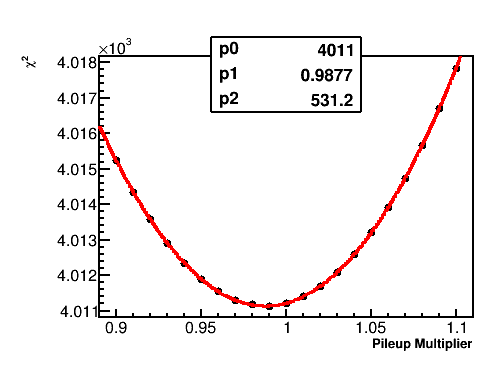
\includegraphics[width=\textwidth]{TMethod_Chi2_Vs_PileupMultiplier_Canv}
        \caption{T-Method \chisq versus pileup multiplier. The parabolic fit equation used was $y = p_{2}(x - p_{1})^{2} + p_{0}.$}
    \end{subfigure}% %you need this % here to add spacing between subfigures
    \hspace{1cm}
    \begin{subfigure}[t]{0.45\textwidth}
        \centering
        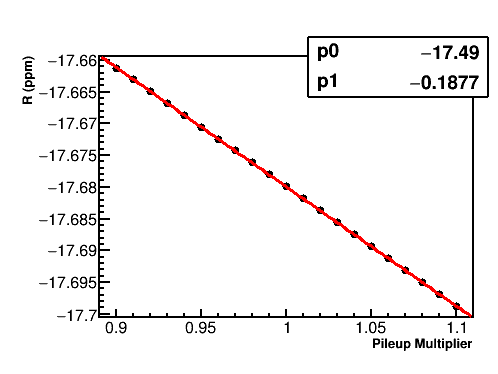
\includegraphics[width=\textwidth]{TMethod_R_Vs_PileupMultiplier_Canv}
        \caption{T-Method $R$ versus pileup multiplier. The parameter $p_{1}$ gives the sensitivity of $R$ to the value of the pileup multiplier, with units in ppm.}
    \end{subfigure}

    \begin{subfigure}[t]{0.45\textwidth}
        \centering
        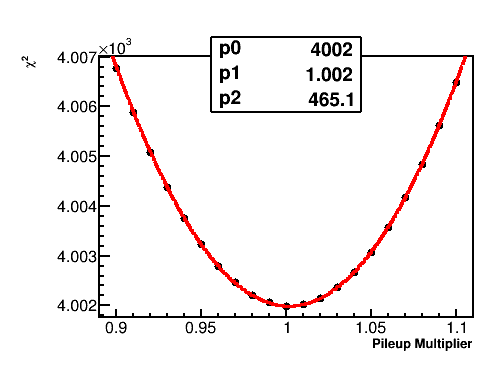
\includegraphics[width=\textwidth]{FullRatio_Chi2_Vs_PileupMultiplier_Canv}
        \caption{R-Method \chisq versus pileup multiplier. The parabolic fit equation used was $y = p_{2}(x - p_{1})^{2} + p_{0}.$}
    \end{subfigure}% %you need this % here to add spacing between subfigures
    \hspace{1cm}
    \begin{subfigure}[t]{0.45\textwidth}
        \centering
        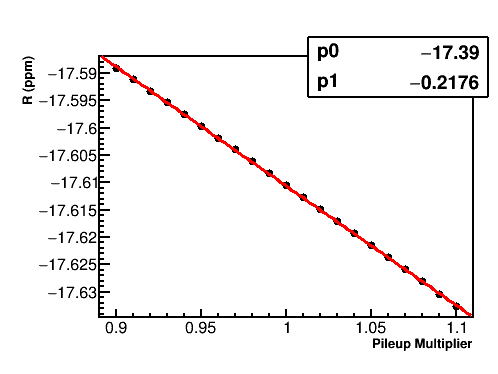
\includegraphics[width=\textwidth]{FullRatio_R_Vs_PileupMultiplier_Canv}
        \caption{R-Method $R$ versus pileup multiplier. The parameter $p_{1}$ gives the sensitivity of $R$ to the value of the pileup multiplier, with units in ppm.}
    \end{subfigure}
\caption[Pileup multiplier scan]{Pileup multiplier scan. Data are from the 9d dataset.}
\label{fig:PMscan}
\end{figure}



\begin{table}
\centering
\renewcommand{\arraystretch}{1.2}
\begin{tabularx}{0.65\linewidth}{@{\extracolsep{\fill}}XYY}
  \hline
    \multicolumn{3}{c}{\textbf{Systematic Error due to Pileup Amplitude}} \\
  \hline\hline
    Dataset & \thead{T-Method} & \thead{R-Method} \\
  \hline
    60h & 21.7 & 19.9 \\
    HighKick & 11.4 & 11.4 \\
    9d & 8.1 & 10.1 \\ 
    Endgame & 10.1 & 9.4 \\
  \hline
\end{tabularx}
\caption[Systematic error due to pileup amplitude]{Systematic error due to the pileup amplitude. Units are in ppb.}
\label{tab:systematicError_pileupMultplier}
\end{table}



\subsection{Cluster Time Model}

\subsection{Cluster Energy Model}

\subsection{Rate Error}

\subsection{Unseen Pileup}

\subsection{Triple Pileup Correction}






